% The study's challenges
%% The importance of energy and energy storage
En 2019, la consommation mondiale d'énergie finale a doublé par rapport à 1973 et a dépassé la barre des \qty{400}{\exa \joule}, dont \qty{19.7}{\percent} d'électricité \cite{birol_key_nodate}.\\
Les énergies renouvelables sont une des solutions pour répondre à cette demande croissante d'électricité tout en respectant l'environnement. Cependant, les périodes de production ne coïncidant pas nécessairement avec les périodes de consommation -- le cycle diurne étant un exemple -- il est nécessaire de pouvoir stocker efficacement l'énergie produite en attendant qu'elle soit consommée.

%% Presenting the SCs
Les électrodes capacitives sont les composants maîtres d'appareils comme les supercondensateurs, constituant une bonne piste pour l'avenir du stockage d'énergie. Elles peuvent être composées de charbon actif sur aluminium, séparées par une membrane perméable et plongées dans un électrolyte. Ceci permet le déplacement des charges d'une électrode à l'autre lorsque l'appareil est en charge ou en décharge sans réactions d'oxydoréduction comme pour les batteries (\autoref{fig:schema_supercondensateur}).\\
Grâce à ce fonctionnement, les supercondendateurs se situent entre les batteries et les condensateurs en termes de densité d'énergie et de puissance, et leur utilisation est répandue pour les véhicules électriques, systèmes d'alimentation sans fil ou encore appareils portables.

\begin{figure}[h!]
    \centering
    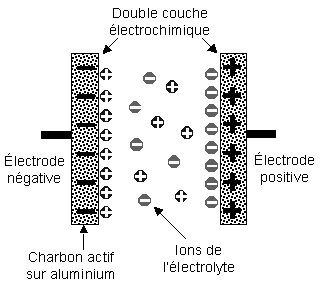
\includegraphics[height = 6 cm]{supercondensateur.png}
    \caption{Schéma d'un supercondensateur}
    \label{fig:schema_supercondensateur}
\end{figure}

% Presenting the state of the art
Plusieurs études ayant des sujets connexes ont déjà été réalisées pour mieux comprendre le comportement des supercapaciteurs, notamment à l'échelle atomique : la densité relative d'ions de l'électrolyte et le potentiel peuvent être ciblés pour étudier la structure de la Double Couche Électrique (\edl{})\cite{jiang_molecular_2016}, ou encore la densité d'ions et de charges pour étudier l'adsorption des ions à l'interface électrode/électrolyte\cite{cole_ion_2011}.
Ces deux études ont été menées sur des électrodes de graphène, avec des électrolytes aqueux. Pour ces systèmes, les interactions ont été modélisées à l'aide de potentiel non-réactifs, et la différence de potentiel entre les électrodes a été contrôlée en définissant les charges de l'ensemble des atomes des électrodes séparément.
Pour cette étude, nous voulons adopter des méthodes quelque peu différentes : en utilisant un potentiel réactif pour les interactions entre les particules [\reaxff{}], et en contrôlant directement le voltage entre les électrodes [\echemdid{}].

% Presenting the problem
La structure des électrodes peut s'avérer très complexe\cite{bo_design_2018}\cite{iro_brief_2016}, en effet les matériaux les plus souvent utilisés pour fabriquer de tels composants sont très poreux : avec des surfaces spécifiques atteignant les \qty{3000}{\square \meter \per \gram}, complexifiant ainsi la structure à cause d'une très large distribution de pores : pouvant comprendre des micropores ($< \qty{2}{\nano\meter}$), des mésopores (\qtyrange[range-units = single]{2}{50}{\nano \meter}) et des macropopres ($> \qty{50}{\nano \meter}$) ; et une grande présence de défauts structurels : comme des atomes de carbone manquants ou substitués par des atomes d'autres types, ou encore des atomes d'autres types ajoutés à la suface de la structure.
Ainsi, nous avons préféré étudier un système modèle [simplifié] pour mieux comprendre la diffusion des charges dans des électrodes en présence d'un défaut simple, puis de deux défauts, etc..

% Presenting the plan
Dans un premier temps, nous discutons des méthodes et outils que nous utilisons dans nos simulations, à savoir : le potentiel réactif \reaxff{}\cite{van_duin_reaxff_2001}\cite{russo_atomistic-scale_2011}\cite{senftle_reaxff_2016}, et la mise en place de la polarisation du système à l'aide d'\echemdid{}\cite{onofrio_voltage_2015}.
Puis, nous présentons le système modèle : ses caractéristiques, sa construction et sa mise en place.
Enfin, nous présentons les résultats obtenus et observations faites lors de cette étude, notamment par rapport à l'adsorption des ions à la surface des électrodes, l'influence de leurs défauts, et la répartition des charges en leur sein.

